\documentclass[android.tex]{subfiles}
\usepackage{subfiles}
\documentclass[12pt,oneside]{memoir} 
\usepackage[latinica]{matfmaster} 

%-----------------------------------------------------------------------------------------
\usepackage{listings}
\usepackage{xcolor}

\definecolor{codegreen}{rgb}{0,0.6,0}
\definecolor{codegray}{rgb}{0.5,0.5,0.5}
\definecolor{codepurple}{rgb}{0.58,0,0.82}
\definecolor{backcolour}{rgb}{0.95,0.95,0.92}

\lstdefinestyle{mystyle}{
    backgroundcolor=\color{backcolour},   
    commentstyle=\color{codegreen},
    keywordstyle=\color{magenta},
    numberstyle=\tiny\color{codegray},
    stringstyle=\color{codepurple},
    basicstyle=\ttfamily\footnotesize,
    breakatwhitespace=false,         
    breaklines=true,                 
    captionpos=b,                    
    keepspaces=true,                 
    numbers=left,                    
    numbersep=5pt,                  
    showspaces=false,                
    showstringspaces=false,
    showtabs=false,                  
    tabsize=2
}

\lstset{style=mystyle}
%-----------------------------------------------------------------------------------------

\begin{document}

Pod Android aplikacijom se smatra bilo koja aplikacija koja se pokreće na uređaju sa OS-om Android. Programiranje ovih aplikacija je moguće u mnogim programskim jezicima, dok se zvaničnim smatraju programski jezici Java i Kotlin \cite{sajt:kotlin}. U nastavku će biti reči o programiranju u programskom jeziku Java.

Kreiranje Android aplikacija ne bi bilo moguće bez njenih osnovnih komponenti. Svaka komponenta ima svoje karakteristike, slučajeve upotrebe kao i funkcije koje vrši. Moguće je i poželjno kombinovati ih u aplikaciji. Svaka komponenta koje se kreira u aplikaciji mora da se navede u datoteci \textit{AndroidManifest.xml}. Četiri osnovne komponente su:

\begin{enumerate}
\item Aktivnosti (eng. \textit{activity})
\item Servisi (eng. \textit{service})
\item Prijemnici (eng. \textit{broadcast receiver})
\item Provajderi sadržaja (eng. \textit{content provider})
\end{enumerate}

\subsection{Datoteka AndroidManifest.xml}
\label{sec:manifest}
Glavna datoteka bez koje nijedna Android aplikacija ne može da postoji je \textit{AndroidManifest.xml}. Pomoću ove XML datoteke OS Android i njegovi alati za izgradnju aplikacija (eng. \textit{build tools}) dobijaju sve potrebne informacije za instalaciju i pokretanje aplikacije. K\^{o}d počinje navođenjem verzije XML-a i kodne sheme, nakon čega sledi etiketa (eng. \textit{tag}) \textit{<manifest>} u okviru kog se piše ceo k\^{o}d. Obavezni deo koda je etiketa \textit{<application>}. Pregled osnovnih elemenata i njihovih opisa može se videti u kodu \ref{lst:manifest}. Više informacija o elementnima i njihovim opcijama može se pronaći na vebu \cite{sajt:manifest}.

\lstinputlisting[language=XML, caption= {Primer \textit{AndroidManifest.xml}, izvor: \cite{sajt:manifest}}, label = {lst:manifest}]{Manifest.xml}



\subsection{Aktivnosti}
Aktivnosti predstavljaju jedan prikaz grafičkog korisničkog interfejsa (eng. \textit{Graphical User Interface}) na ekranu. Ne postoji ograničeni broj aktivnosti koje jedna aplikacija može imati, takođe moguće je da postoje aplikacije bez aktivnosti. Za razliku od mnogih programskih jezika gde pokretanje aplikacije počinje pozivom metoda \textit{main()} i uvek od istog mesta, Android aplikacije ne moraju uvek započinjati na istom mestu. Uglavnom Android aplikacije imaju jedan početni ekran koji se naziva \textit{Main Activity} i  koji se pokreće pri pokretanju aplikacije i više dodatnih koji su logički povezani sa početnim. Logika iza koje stoji ovaj koncept je da je korisniku omogućeno da pokrene različite delove aplikacije u zavisnosti od trenutnih potreba. Jedan primer koji ovo ilustruje je kada korisnik klikne na obaveštenje aplikacije za dostavu hrane da je hrana koju je naručio u putu, aplikacija će otvoriti aktivnost koja prikazuje mapu za praćenje, a ne početnu stranu za izbor restorana.

Svaka aktivnost ima četiri osnovna stanja: 
\begin{enumerate}
    \item Trajanje (eng. \textit{running})
    \item Mirovanje (eng. \textit{paused})
    \item Zaustavljeno (eng. \textit{stopped})
    \item Uništeno (eng. \textit{destroyed})
\end{enumerate}
Pri implementaciji svaka aktivnost mora da ima svoje ime i da nasleđuje klasu \textit{Activity}. Ova klasa pruža metode koji prate osnovna stanja životnog ciklusa aktivnosti: \textit{onCreate(), onStart(), onPause(), onResume(), onStop(), onDestroy() i onRestart()} \cite{book:and9cookbook}. Ove metode je potrebno predefinisati (eng.~\textit{override}) kako bi se definisala ponašanja aktivnosti za svaku promenu njenog stanja. Životni ciklus aktivnosti je prikazan na slici \ref{fig:zivotniCiklus}.


\begin{figure}[!ht]
  \centering
  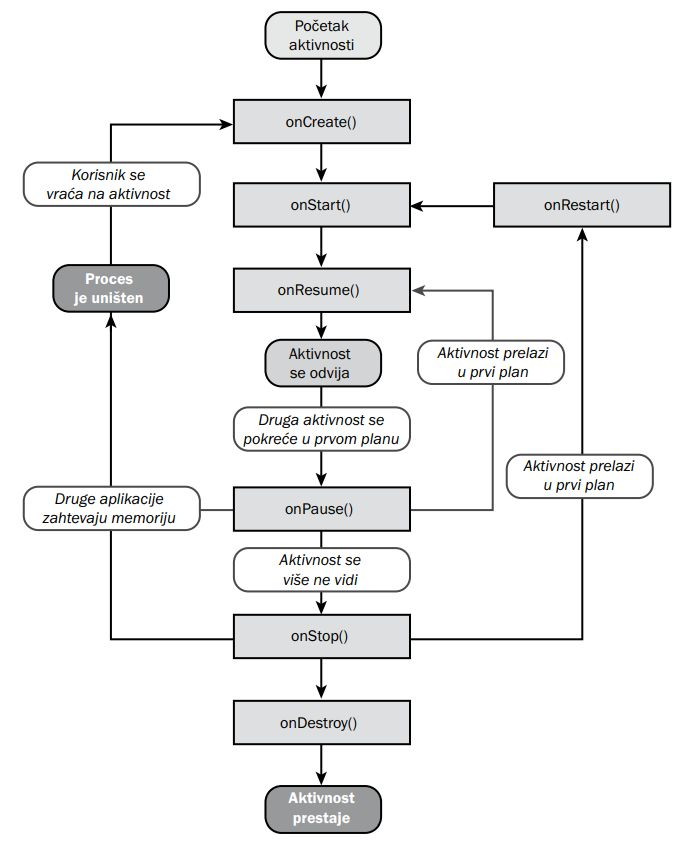
\includegraphics[width=0.9\textwidth]{Android/lifecycle-srpski.jpg}
  \caption{Životni ciklus aktivnosti, slika preuzeta sa \cite{sajt:zivotniCiklusSlika}}
  \label{fig:zivotniCiklus}
\end{figure}


Metod \textit{onCreate()} je metod u kojem se nalazi logika koja je potrebna da se izvrši pri prvom pokretanju aktivnosti. U njemu je potrebno uraditi sve inicijalizacije osnovnih komponenti aktivnosti kao i inicijalizaciju statičkih promenljivih, stavljanje podataka u liste... Iz ovog metoda mora se pozvati metod \textit{setContentView()} koji određuje prikaz grafičkog korisničkog interfejsa. Nakon izvršavanja \textit{onCreate() }metoda uvek se poziva metod \textit{onStart()}.

Metod \textit{onStart() }vodi računa o svemu što je potrebno da aktivnost bude vidljiva korisniku. Aplikacija ovde priprema aktivnost da bude prikazana korisniku. Može se registrovati prijemnik da osluškuje promene koje bi izmenile grafički korisnički interfejs. Metodi koji prate \textit{onStart()} su \textit{onResume() }ili \textit{onStop()}.

Metod \textit{onPause()} se poziva u trenutku kada se primeti da korisnik više neće koristiti tu aktivnost. S obzirom da se njeno izvršavanje dešava u momentu kada je aktivnost još uvek vidljiva korisniku sve što se izvršava u metodi mora biti brzo jer sledeća aktivnost neće biti nastavljena dok se metod ne završi. Ovde treba prekinuti sve što nije potrebno da se izvršava kada je aktivnost u stanju mirovanja. Ovaj metod prate metodi \textit{onResume()} ukoliko se fokus vrati na ovu aktivnost ili \textit{onStop() }ukoliko je aktivnost nevidljiva korisniku.

Metod \textit{onResume()} se poziva kada aktivnost počinje da ima interakciju sa korisnikom.

Metod \textit{onStop()} se poziva kada god aktivnost više nije vidljiva korisniku što može biti zbog toga što je pokrenuta nova aktivnost ili jer se trenutna aktivnost uništava. Neki od čestih primera kada se koristi implementacija ove metode su osvežavanje korisničkog interfejsa i zaustavljanje animacija ili muzike. Ukoliko se aktivnost vraća interakciji sa korisnikom pozvaće se metod \textit{onRestart()}, u suprotnom metod \textit{onDestroy()}.

Metod \textit{onDestroy()} je poslednji poziv i može se desiti iz dva razloga. Prvi, jer se aktivnost završava. Drugi, da se privremeno gasi aktivnost radi čuvanja memorijskog prostora. Koji se razlog desio može se saznati pomoću metode \textit{isFinishing()}.

Metod \textit{onRestart() }se poziva nakon što je aktivnost stopirana, a pre njenog ponovnog prikaza. Tu možemo uraditi eventualne ponovne inicijalizacije ili neke izmene korisničkog interfejsa pre nego što bude ponovo pozvan metod \textit{onStart()}.

\subsection{Servisi}
Servis je komponenta koja izvršava svoje zadatke u pozadini i najčešće se koriste za zadatke koji se dugo izvršavaju i koji bi usporili aplikaciju ako bi se izvršavali na glavnoj niti. Servisi nemaju grafički korisnički interfejs, ali mogu da komuniciraju sa ostalim komponentama \cite{book:hellman}. U zavisnosti od tipa zadatka koji se očekuje da servis izvrši, kao i dužine trajanja izvršavanja razlikuju se tri vrste servisa:
\begin{description}
    \item \textit{Pozadinski} (eng. \textit{background}) servisi ne obaveštavaju korisnika ni na koji način o zadacima koje izvršavaju zbog toga što za njihovo izvršavanje nije potrebna nikakva interakcija sa korisnikom. Primer je sinhronizovanje podataka u unapred određeno vreme.  
    \item \textit{Vidljivi} (eng. \textit{foreground}) su servisi za koje korisnici znaju da se izvršavaju tako što servis pomoću obaveštenja obaveštava korisnika o svom izvršavanju. Korisniku se daje mogućnost da pauzira ili u potpunosti zaustavi proces koji se izvršava. Primer ovog servisa je preuzimanje datoteka.
    \item \textit{Vezani} (eng. \textit{bound}) servisi se izvršavaju kada je neka komponenta aplikacije povezana sa servisom, odnosno dokle god postoji neka komponenta kojoj je potrebno izvršavanje zadataka koje dati servis izvršava.
\end{description}

Na osnovu životnog ciklusa servisa razlikujemo pokrenute (eng. \textit{started}) servise i povezane (eng. \textit{bounded}). Pokrenut servis se inicijalizuje pozivom \textit{startService()} metode, a zaustavlja kada komponenta pozove metod \textit{stopService() }ili ukoliko sam servis pozove metod \textit{stopSelf()}. Povezani servisi se mogu doživeti kao klijent-server orgqanizacija zato što komponente mogu da šalju zahteve servisu, kao i da dohvataju rezultate. U trenutku kada neka komponenta pozove metod \textit{bindService()} i time se poveže sa servisom servis se smatra povezanim, a tek kada se sve komponente aplikacije koje su bile povezane sa njim oslobode pozivom \textit{unbindService()} servis prestaje sa radom. Svi navedeni metodi su iz klase \textit{Service} koju je neophodno da svaki servis nasledi pri implementaciji.


\subsection{Prijemnici}
Prijemnici služe da osluškuju sistemska obaveštenja kao i obaveštenja od strane drugih aplikacija na uređaju ili drugih delova iste aplikacije. Da bi mogao da izvršava svoju funkciju potrebno je da prijemnik bude registrovan da osluškuje određene namere (eng. \textit{intent}). Moguće je da jedan prijemnik osluškuje više različitih namera i u zavisnosti od namere da izvršava različite operacije. Neki od primera upotrebe sistemskih prijemnika su prijemnik za procenat baterije, prijemnik za alarm i prijemnik za SMS poruke \cite{book:mzivkovic}. 

\subsection{Provajderi sadržaja}
Provajderi sadržaja obezbeđuju skladištenje podataka aplikacije. Pored samog skladištenja njihova uloga je i da omoguće drugim aplikacijama da pristupe sadržaju ukoliko imaju prava za to. Samo skladištenje je moguće da bude pomoću \textit{SQLite} baza podataka, datoteka ili na mreži. Sa strane implementacije aplikacija koja želi da deli svoje podatke mora da koristi klasu \textit{ContentProvider} i kreira interfejs prema tim podacima. Druga aplikacija da bi mogla da  koristi te podatke mora da napravi instancu objekta klase \textit{ContentResolver} sa svim metodama koje prva aplikacija poseduje. 

\subsection{Namere}
\label{sec:namere}
Namera predstavlja objekat koji slanjem poruke zahteva da drugi deo aplikacije ili druga aplikacija izvrši neku akciju. Najčešće su tri upotrebe namera: pokretanje aktivnosti, pokretanje servisa i slanje poruka (eng. \textit{broadcast}). Implementacija se vrši pomoću klase \textit{Intent} i potrebno je kreirati novi objekat \cite{sajt:androidDevelopers}. 






\end{document}